


\subsection{Grid Options}
	
\begin{pgfplotsxykeylist}{\x minorgrids=\mchoice{true,false} (initially true),\x majorgrids=\mchoice{true,false} (initially true),grid=\mchoice{minor,major,both,none} (initially both)}
Enables/disables different grid lines. Major grid lines are placed at the normal tick positions (see |xmajorticks|) while minor grid lines are placed at minor ticks (see |xminorticks|). 

This example employs the coordinates defined on page~\pageref{page:plotcoords:src}.
\begin{codeexample}[]
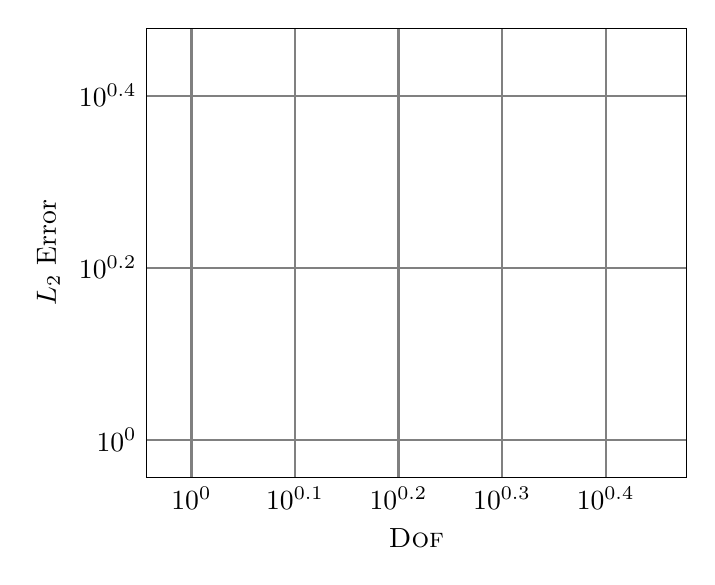
\begin{tikzpicture}
\begin{loglogaxis}[
	xlabel={\textsc{Dof}},
	ylabel={$L_2$ Error},
	grid=major
]
% see above for this macro:
\plotcoords
\end{loglogaxis}
\end{tikzpicture}
\end{codeexample}

\begin{codeexample}[]
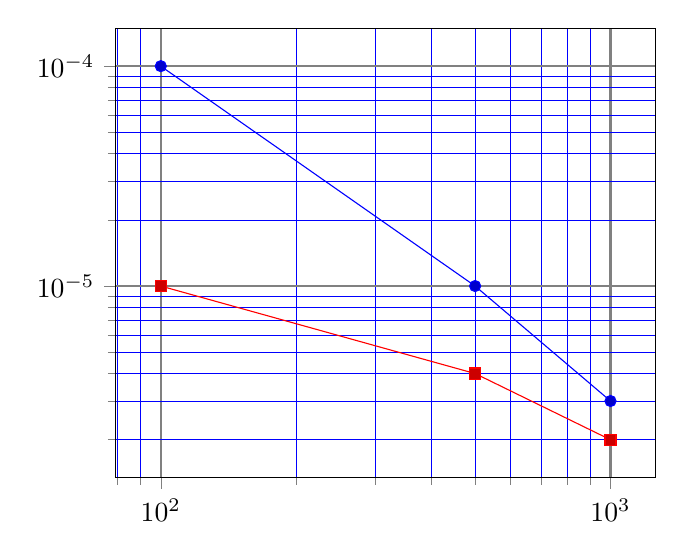
\begin{tikzpicture}
\begin{loglogaxis}[
	grid=both,
	tick align=outside,
	tickpos=left]
\addplot coordinates 
	{(100,1e-4) (500,1e-5) (1000,3e-6)};
\addplot coordinates 
	{(100,1e-5) (500,4e-6) (1000,2e-6)};
\end{loglogaxis}
\end{tikzpicture}
\end{codeexample}

Grid lines will be drawn before tick lines are processed, so ticks will be drawn on top of grid lines. You can configure the appearance of grid lines with the styles
\begin{codeexample}[code only]
\pgfplotsset{every axis grid/.style={style=help lines}}
\pgfplotsset{every minor grid/.append style={color=blue}}
\pgfplotsset{every major grid/.append style={thick}}
\end{codeexample}
\noindent and/or the keys |grid style=|\marg{keys}, |minor grid style=|\marg{keys} and |major grid style=|\marg{keys}.
\end{pgfplotsxykeylist}


\subsection{Accessing Axis Coordinates for Annotations}
\label{sec:axis:coords}%
\begin{coordinatesystem}{axis cs}
\PGFPlots\ provides a new coordinate system for use inside of an axis, the ``axis coordinate system'', |axis cs|.

It can be used to draw any \Tikz-graphics at axis coordinates. It is used like
\begin{codeexample}[code only]
\draw 
   (axis cs:18943,2.873391e-05) 
|- (axis cs:47103,8.437499e-06);
\end{codeexample}
\begin{codeexample}[]
\tikzstyle{every pin}=[fill=white,
	draw=black,
	font=\footnotesize]
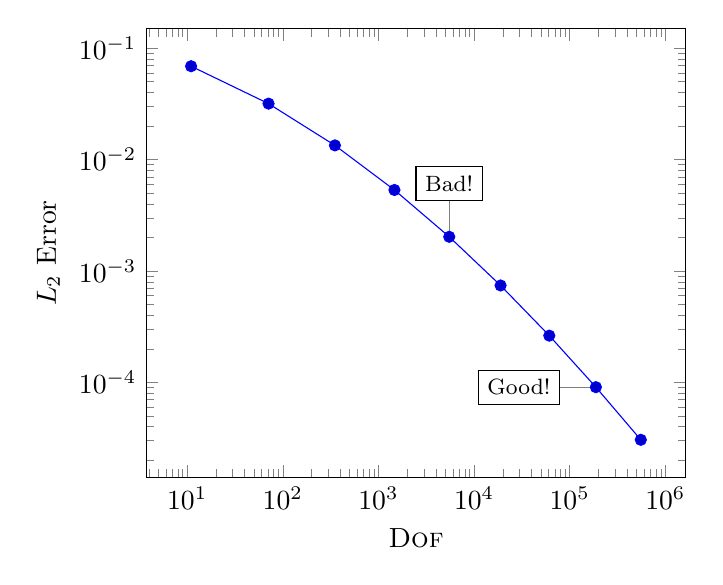
\begin{tikzpicture}
	\begin{loglogaxis}[
		xlabel={\textsc{Dof}},
		ylabel={$L_2$ Error}]

	\addplot coordinates {
		(11,     6.887e-02)
		(71,     3.177e-02)
		(351,    1.341e-02)
		(1471,   5.334e-03)
		(5503,   2.027e-03)
		(18943,  7.415e-04)
		(61183,  2.628e-04)
		(187903, 9.063e-05)
		(553983, 3.053e-05)
	};

	\node[coordinate,pin=above:{Bad!}] 
		at (axis cs:5503,2.027e-03) {};
	\node[coordinate,pin=left:{Good!}] 
		at (axis cs:187903,9.063e-05)	{};
	\end{loglogaxis}
\end{tikzpicture}
\end{codeexample}

\begin{codeexample}[]
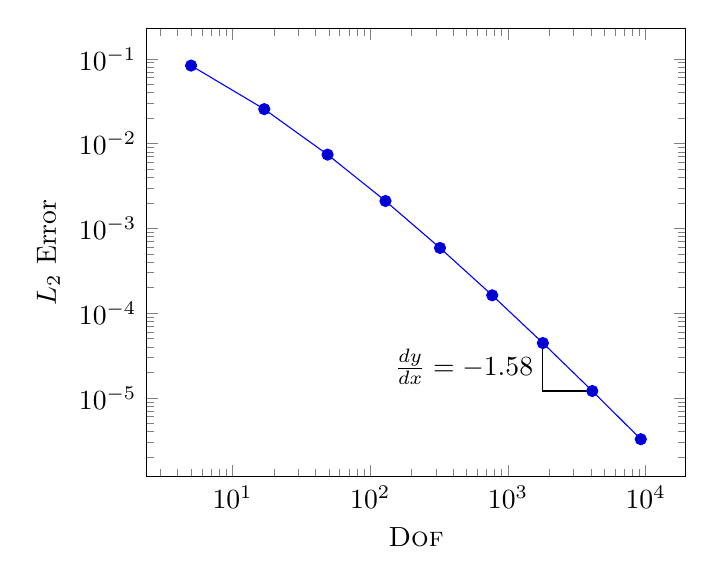
\begin{tikzpicture}
\begin{loglogaxis}[
	xlabel=\textsc{Dof},
	ylabel=$L_2$ Error
]
\draw 
		(axis cs:1793,4.442e-05)
	|-  (axis cs:4097,1.207e-05)
	node[near start,left] 
	{$\frac{dy}{dx} = -1.58$};

\addplot coordinates {
	(5,    8.312e-02)
	(17,   2.547e-02)
	(49,   7.407e-03)
	(129,  2.102e-03)
	(321,  5.874e-04)
	(769,  1.623e-04)
	(1793, 4.442e-05)
	(4097, 1.207e-05)
	(9217, 3.261e-06)
};
\end{loglogaxis}
\end{tikzpicture}
\end{codeexample}

\paragraph{Attention:} Whenever you draw additional graphics, consider using |axis cs|! It applies any logarithms, data scaling transformations or whatever \PGFPlots\ usually does!

There is also a low--level interface to access the transformations and coordinates, see section~\ref{sec:pgfplots:lowlevel} on page~\pageref{sec:pgfplots:lowlevel}.
\end{coordinatesystem}

\begin{coordinatesystem}{rel axis cs}
The ``relative axis coordinate system'', |rel axis cs|, uses the complete axis vectors as units. That means `$x=0$' denotes the point on the lower $x$ axis range and `$x=1$' the point on the upper $x$ axis range.

\pgfplotsexpensiveexample
\begin{codeexample}[]
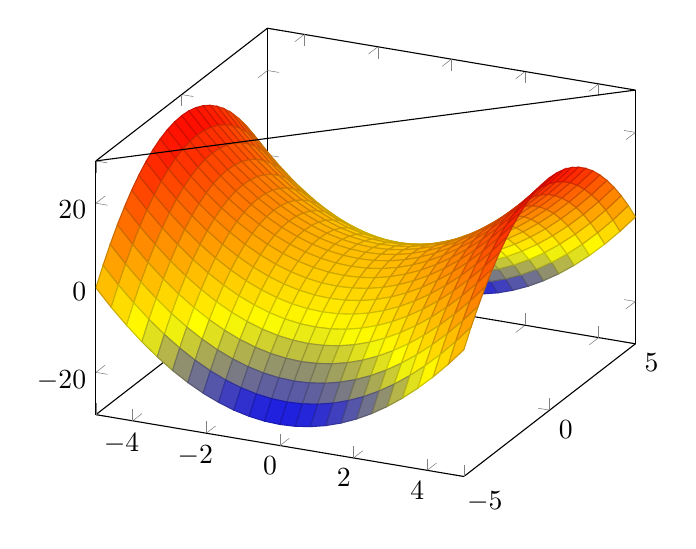
\begin{tikzpicture}
\begin{axis}

	\addplot3[surf] {x^2 - y^2};
	\draw  (rel axis cs:0,0,1) 
		-- (rel axis cs:1,1,1);
\end{axis}
\end{tikzpicture}
\end{codeexample}

\pgfplotsexpensiveexample
\begin{codeexample}[]
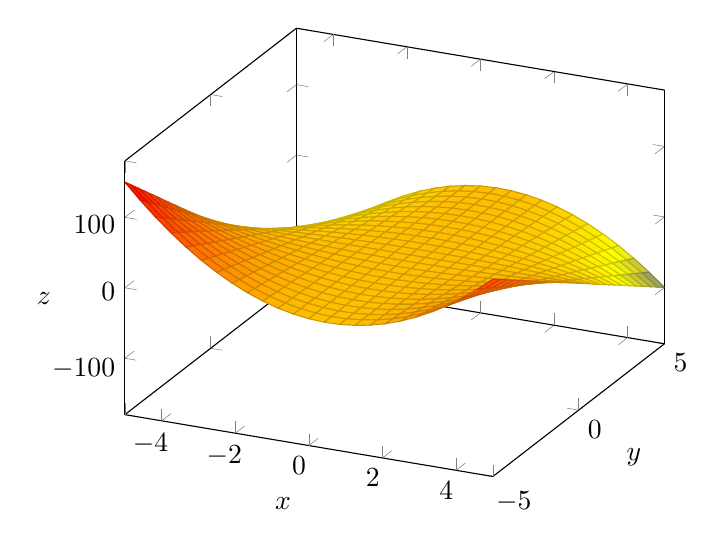
\begin{tikzpicture}
\begin{axis}[
	xlabel=$x$,
	ylabel=$y$,
	zlabel=$z$,
	every axis x label/.style={
		at={(rel axis cs:0.5,-0.15,-0.15)}},
	every axis y label/.style={
		at={(rel axis cs:1.15,0.5,-0.15)}},
	every axis z label/.style={
		at={(rel axis cs:-0.15,-0.15,0.5)}},
]

	\addplot3[surf] {x*(1-x)*y};
\end{axis}
\end{tikzpicture}
\end{codeexample}

There is also a low--level interface to access the transformations and coordinates, see section~\ref{sec:pgfplots:lowlevel} on page~\pageref{sec:pgfplots:lowlevel}.
\end{coordinatesystem}

\begin{predefinednode}{current plot begin}
	This coordinate will be defined for every plot and can be used is \meta{trailing path commands} or after a plot. It is the first coordinate of the current plot.	
\end{predefinednode}

\begin{predefinednode}{current plot end}
	This coordinate will be defined for every plot. It is the last coordinate of the current plot.	
\end{predefinednode}

